\chapter{Approach}
\label{ch:approach}

\section{Overall Approach}
To answer the three RQs mentioned in section~\ref{sec:intro:objectives} we want to compare some models find in literature. Mainly the fair Bayesian network and the fair tree classifiers. These should be evaluated on datasets used in machine learning research. We then will perform experiments evaluating the performance metrics of the models, as well as new performance metrics reflecting fairness. After collecting the data on the performance of the models, hypothesis testing will be done to evaluate whether the differences are significant.

\section{Python Code Repository: Forseti}

\begin{figure}
    \centering
    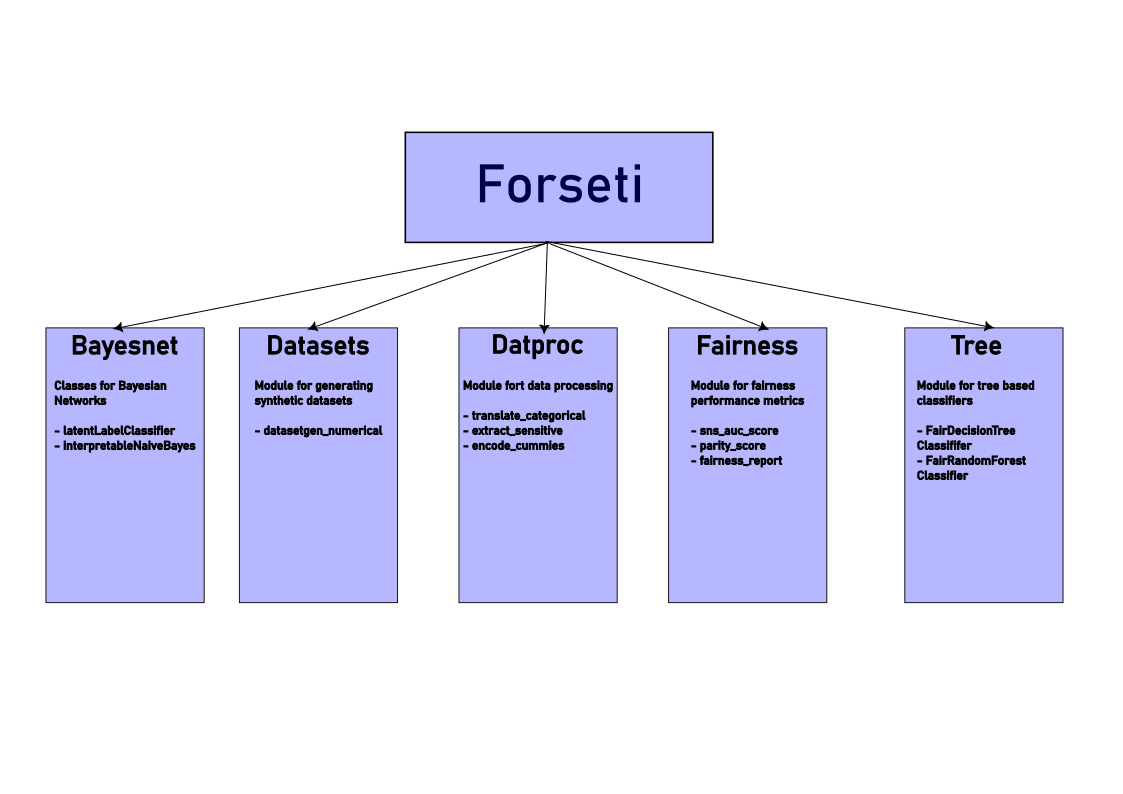
\includegraphics[width=\linewidth]{figures/tegning.png}
    \caption{Setup of Forseti Python Module}
    \label{fig:forseti}
\end{figure}

We manage the code through GitHub, a python module named Forseti as well as some Jupyter notebooks. In figure \ref{fig:forseti} the structure of the module is shown. It has the following modules:

\begin{itemize}
    \item Bayesnet: This module contains classes of Bayesian networks.
    \item Datasets: This module contains functions for generating synthetic datasets.
    \item Datproc: Data processing module.
    \item Fairness: Fairness metrics and fairness reports.
    \item Tree: Tree based methods and classifiers.
\end{itemize}

The code and its documentation is available at GitHub\footnote{\url{https://github.com/bcwein/forseti}}. The aim of organising the code in such a way was to make it as easy as possible to let others run the code on their own systems. How to do this is described in the next section.

\subsection{Setup}

The environment used in Forseti is available in the file \emph{environment.yml} and one can setup the environment using Anaconda. See the documentation \footnote{\url{https://docs.conda.io/projects/conda/en/latest/user-guide/tasks/manage-environments.html\#creating-an-environment-from-an-environment-yml-file}} on how to do this.

If one prefers to not use anaconda, the necessary packages are as follows:

\begin{itemize}
    \item Python
    \item Pytest
    \item Black
    \item Jupyter
    \item ipykernel
    \item Pandas
    \item Seaborn
    \item pip
    \item pgmpy
\end{itemize}

\section{Data Exploration and Selection}

For this thesis, exploration of approaches to achieve fairness and interpretability in machine learning algorithms is the goal. The Adult dataset \footnote{\url{https://archive.ics.uci.edu/ml/datasets/adult}} was selected for this topic. Before beginning on implementing machine learning methods and experiments, some preliminary data exploration is in order.

\subsection{Adult Dataset}

To select the features of interest and as an initial data exploration. We will investigate the correlation between the features and the dependent variable \emph{income}. Since almost all the attributes are categorical, we calculate correlation using dummy variables. Which means, transforming categorical attributes to columns of binary attributes. We then explore which dummy variables have the highest absolute correlations. We interpret the weight of each variable as the absolute sum of its dummies. 

\subsection{COMPAS Dataset}
The COMPAS dataset contains records for defendants from Broward County indicating their jail and prison times, demographics, criminal histories and COMPAS risk scores from 2013 to 2014 \cite{Mehrabi:2021:CSUR}. This dataset is high dimensional with a mix of categorical, numerical and date time columns. For this thesis, the focus has not been to implement the best model out there, but rather compare the fairness between models. Therefore, we have limited ourselves to the following attributes when training our algorithms

\begin{itemize}
    \item Sex: Gender of individual (binary)
    \item Age: Age of individual (positive integer)
    \item Race: Ethnicity of individual (6 categories)
    \item Priors Count: Prior Crimes (positive integer)
    \item Juvenile felony count: Felonies as a juvenile (positive integer)
    \item Juvenile misdemeanour count: Misdemeanours as a juvenile (positive integer)
    \item Juvenile other count: Other charges as a juvenile (positive integer)
    \item Charge degree: Degree of current charge (binary)
    \item Two year recidivism: Whether individual reoffended within two years (binary)
\end{itemize}

We selected these attributes mainly due to these being the only attributes in the dataset that are not recorded after rearrest and were not in a date time format. The point is not to make the best performing classifier, but to compare classifiers with regard to fairness.

\section{Metric for fair machine learning}

Using demographic parity as described in equation~\ref{eq:dempar} is the metric of choice for evaluating the model fairness in this thesis. The main reason for this is that the metric does not assume that the dataset labels are fair. Demographic parity is appropriate to use when we want our predictions to be more in line with a state of nature that we want to see in the world and when we are aware of historical biases that affect the data.~\footnote{\url{https://bit.ly/3Ko10sL}}. In the case of the adult dataset described in section~\ref{sec:adult}, we have the binary sensitive attributes \emph{gender} and the categorical sensitive attribute \emph{race}, both of which are known to experience discrimination in income. 

\begin{figure}
    \centering
    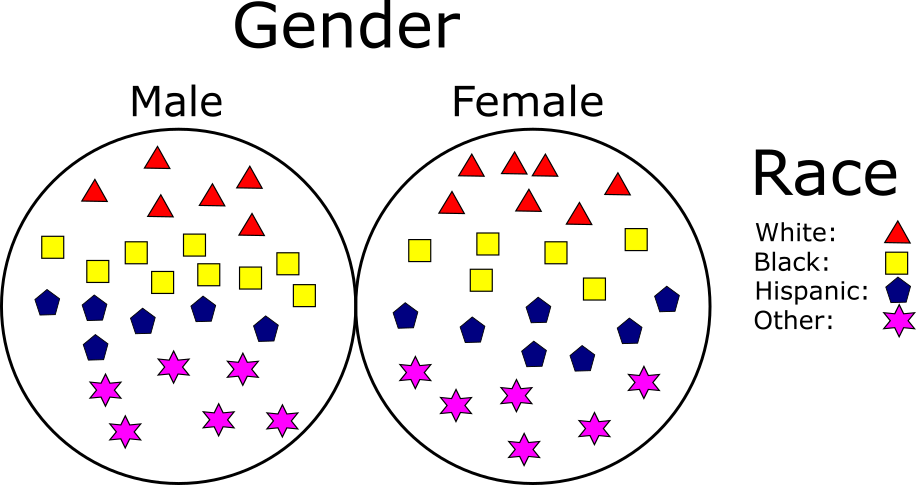
\includegraphics[width=0.7\linewidth]{figures/GroupOverlap.png}
    \caption{Visualisation of overlapping groups.}
    \label{fig:overlap}
\end{figure}

A challenge when working with multiple sensitive attributes and multivariate sensitive attributes is that you get overlapping groups. See figure~\ref{fig:overlap} for an example. There we see that we have the binary attribute \emph{Gender} and the categorical \emph{Race} we have several subgroups, i.e., Black Women, White Male etc. An algorithm can be \emph{independently group fair} when you calculate fairness for each sensitive attribute independently, and/or \emph{intersectional group fair} when you calculate fairness for all subgroups \cite{Yang:2020:CoRR}. In this thesis, we use both approaches to calculate parity. 

\subsection{Scoring Function: Demographic Parity Score}
\label{sec:demparscore}
We defined a new scoring function based on demographic parity in equation~\ref{eq:dempar}, where $\hat{Y}$ is the predictor and $S$ the sensitive attribute. This equation can be generalised to the case where we have a categorical sensitive attribute with $K$ classes.

$$
P(\hat{Y} | S_i) = P(\hat{Y} | S_j) \qquad i, j \in \{0, \dots, K-1\}, \qquad i \neq j
$$

When calculating the probabilities, we want to condense these probabilities to a single metric between $0$ and $1$. I.e, when we have the likelihood of a positive outcome for the different classes of a sensitive attribute in a list of  probabilities $L$ like so

$$
L =\{ P(\hat{Y}=1 | S=0), \dots, P(\hat{Y}=1 | S=K-1) \}
$$

We want a function $f$ that takes such a list and maps it to a real number between $0$ and $1$

$$
f: L \rightarrow [0, 1]
$$

It is important that this function works for a list of likelihoods of arbitrary length, since we want to evaluate demographic parity for both binary and categorical sensitive attributes as well as all intersections of the sensitive attributes. Given the definition of demographic parity, we want the likelihoods to be as equal as possible. The scoring function derived is shown below

$$
f = 1 - 2\sigma(L)
$$

\begin{table}[]
    \centering
    \begin{tabular}{|l|l|}
        \hline
        $L$                 & $f$  \\ \hline
        {[}0.5, 0.5{]}      & 1    \\ \hline
        {[}0.6, 0.7{]}      & 0.9  \\ \hline
        {[}0.6, 0.8, 0.4{]} & 0.67 \\ \hline
        {[}0, 1, 0, 1{]}    & 0    \\ \hline
    \end{tabular}
    \caption{Example of values of $f$ given different lists of likelihoods.}
    \label{tab:scorefunc}
\end{table}

where $\sigma$ denotes the standard deviation. We plotted the scoring function in figure~\ref{fig:scorefunc}. The scoring function receives a list of two probabilities which slowly diverges from being equal at $0.5$ to the complete opposite, i.e $[0, 1]$. When the probabilities are equal, the score is 0 and if they are very different, the score is 0. See the examples of scores in table~\ref{tab:scorefunc}

\begin{figure}
    \centering
    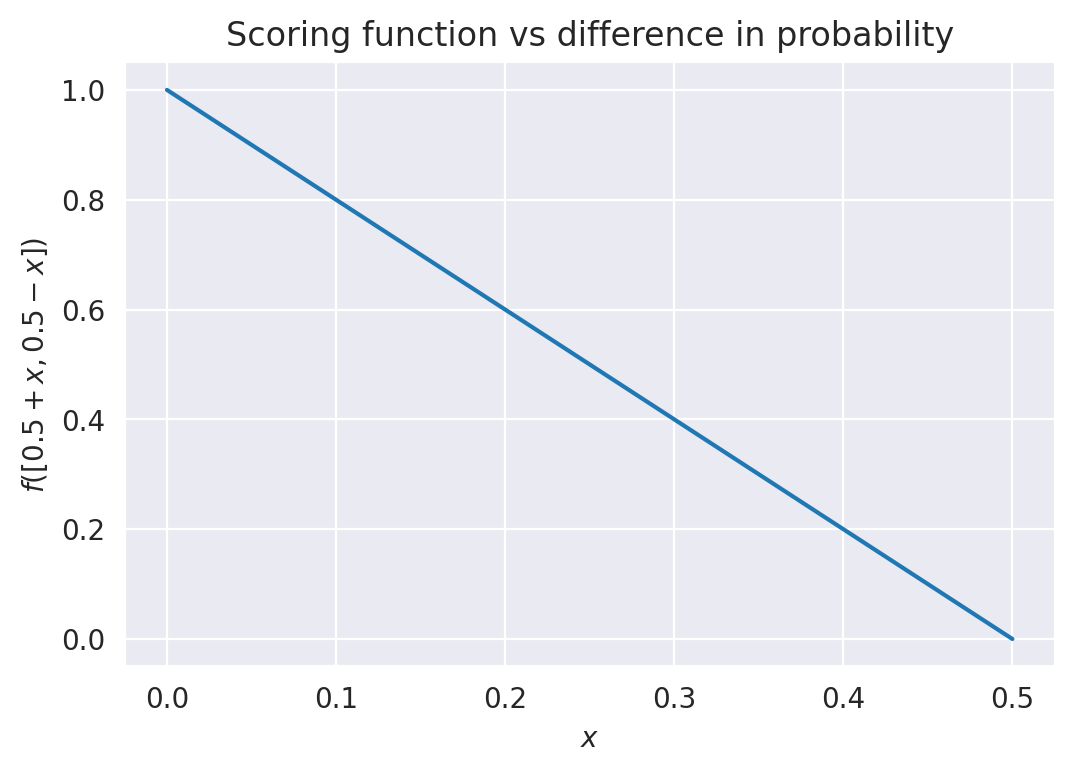
\includegraphics[width=0.7\linewidth]{figures/Parity_metric.png}
    \caption{Scoring function for a list of two diverging probabilities}
    \label{fig:scorefunc}
\end{figure}

\section{Fair Bayesian Network}
\label{sec:fairbayesiannetwork}
Based on the fair Bayesian network described by \citet{Choi:2021:AIII}, the following algorithm was derived.

\begin{algorithm}
    \caption{Latent Label Classifier Training}
    \begin{algorithmic}
        \REQUIRE $D = $ Training Dataset, $S = $ Sensitive Attributes, $L = $ attribute to predict. $t = $ tolerance for expectation maximisation.
        \ENSURE $M = $ Trained Bayesian network.
        \STATE Set of blacklisted nodes: $B = \{(x, y) \quad \forall x \in D.\text{columns}, \quad \forall y \in S\}$
        \STATE $M$.structure $=$ HillClimbSearch($D.$columns $\setminus L$, $B$)
        \STATE $M.$structure$ \cup \{ (x, L) \quad \forall x \in $S$\}$
        \STATE initialise fair node $F$
        \STATE $M.$structure$ \cup \{ (F, x) \quad \forall x \in D.\text{columns}\}$
        \STATE $M.$structure$ \cup \{ (F, L)\}$
        \STATE M.parameters $=$ ExpectationMaximisation($M$.structure, $D$)
        \RETURN M 
    \end{algorithmic}
\end{algorithm}

This method uses two methods implemented in pgmpy \cite{Ankan:2015:SCIPY}. These are Hill Climb Search for learning the structure which is described in section~\ref{HillClimbSearch} and Expectation Maximisation which is described in section~\ref{Expectation Maximization}. The resulting Bayesian network on the adult dataset is shown below in figure~\ref{fig:latentFairClassifierAdult}.

\begin{figure}[h!]
    \centering
    \begin{tikzpicture}[nodes={draw, circle}, ->]
        \node (Race) {$R$};
        \node (Gender) [right=of Race]{$G$};
        \node (Fair) [right=of Gender] {$F$};
        \node (Capital) [below=2cm of Race] {$C$};
        \node (Relationship) [left=of Capital] {$R_e$};
        \node (Education) [left=of Relationship] {$E$};
        \node (Age) [left=of Education] {$A$};
        \node (Marital) [right=of Capital] {$M$};
        \node (Workclass) [right=of Marital] {$W$};
        \node (Hours) [right=of Workclass] {$H$};
        \node (Occupation) [right=of Hours] {$O$};
        \node (Income) [right=of Occupation] {$I$};

        \draw (Fair) -> (Age);
        \draw (Fair) -> (Education);
        \draw (Fair) -> (Relationship);
        \draw (Fair) -> (Capital);
        \draw (Fair) -> (Marital);
        \draw (Fair) -> (Workclass);
        \draw (Fair) -> (Hours);
        \draw (Fair) -> (Occupation);
        \draw (Fair) -> (Income);
        
        \draw (Race) -> (Income);
        \draw (Race) -> (Marital);
        
        \draw (Gender) -> (Relationship);
        \draw (Gender) -> (Marital);
        \draw (Gender) -> (Workclass);
        \draw (Gender) -> (Hours);
        \draw (Gender) -> (Occupation);
        \draw (Gender) -> (Income);
        
        \draw (Age) to  [out=270,in=240] (Hours);
        \draw (Relationship) to  [out=270,in=300] (Age);
        \draw (Relationship) to  [out=270,in=240] (Hours);
        \draw (Marital) to [out=270,in=300] (Age);
        \draw (Marital) to [out=270,in=300] (Relationship);
        \draw (Workclass) to [out=270,in=240] (Occupation);
        \draw (Hours) to [out=270,in=300] (Workclass);
        \draw (Hours) to [out=270,in=240] (Occupation);
        \draw (Occupation) to [out=270, in=300] (Education);
    \end{tikzpicture}
    \caption{latentFairClassifier trained on Adult Dataset. The nodes are $R$: race, $G$: gender, $F$: latent fair labels, $A$: Age, $E$: Education, $R_e$: Relationship, $C$: Capital gain, $M$: Marital Status, $W$: Work class, $H$: Hours-per-week, $O$: Occupation and $I$: Income.}
    \label{fig:latentFairClassifierAdult}
\end{figure}
Inference has been performed by evaluating $P(F | A, E, R_e, C, M, W, H, O)$ on a test dataset of unobserved labels.

\section{Fair Tree Classifier}
The fair tree classifier, described in detail in section~\ref{sec:fairtree}. \citet{Antonio:2021:arXiv} kindly provided their code on GitHub, which made implementing this over to Forseti a bit easier. The code is available in their repository\footnote{\url{https://bit.ly/3x937Nr}}. We added their decision tree classifier and fair random forest classifier classes to Forseti and train and test the models on the same datasets as the fair tree classifier.

\section{Experiment 1: Test Models on COMPAS and Adult Dataset}
\label{sec:AdultAdultFairnessAssessment}
After implementing the Fair Bayesian Network and the Fair Tree Classifier. We wanted to evaluate the models on the Adult Dataset and COMPAS Dataset. To evaluate the models we had to choose some performance metrics. A combination of traditional performance metrics and a fairness score was desired. The fairness score used is the one described in section~\ref{sec:demparscore}. For the traditional metrics there were several pros and cons for each of them. We will go through each one of them and explain the motivation for using that particular scoring method.

\subsection{Accuracy}

We use the accuracy score as implemented in Scikit-Learn. Which follows the following formula

\begin{equation*}
    A(y, \hat{y}) = \frac{1}{n_\text{samples}} \sum_{i=0}^{n_\text{samples} - 1} 1(\hat{y}_i = y_i)
\end{equation*}

Accuracy is a very intuitive coring function for predictions, as it can be interpreted as the ratio of correct classifications. The problem with accuracy as a scoring function is when datasets are imbalanced, the scoring function also suffers and are biased toward the most prominent class.

\subsection{Balanced Accuracy}

Balanced Accuracy is calculated as follows

\begin{equation*}
    BA(y, \hat{y}) = \frac{1}{\sum \hat{w}_i} \sum_i 1(\hat{y}_i = y_i)\hat{w}_i
\end{equation*}

where $\hat{w}_i$ is sample weight of the i-th sample and the weight is adjusted to 

\begin{equation*}
    \hat{w}_i = \frac{w_i}{\sum_j 1(y_j = y_i)w_j}
\end{equation*}

Balanced Accuracy is equal to the arithmetic mean of the sensitivity and specificity in the binary case. Since this accuracy score scales with imbalanced datasets it gives a more clear picture of how well the classifier performs and adjusts if the classifier takes advantage of the imbalance.

\subsection{F1 Score}

The F1 score is defined as the harmonic mean of precision and recall and thus reflect. We chose to add F1 score as it is a commonly used score in machine learning and the score reflects how well the model is able to maximise precision and recall and not have a huge disparity between them. One challenge with F1 score is that it ignores true negatives. 

\subsection{Specificity}

And lastly, we calculate the specificity (true negative rate). Which is calculated from the confusion matrix as follows

\begin{equation*}
    TNR(\hat{y}, y) = \frac{TN}{N}
\end{equation*}

We mainly chose this metric since F1 score ignores true negatives and by having this in our fairness report we have some information with regard to true negatives.

\subsection{ROC Curve}

We also want to calculate the ROC curve and plot it to see the threshold independent performance of the model. This requires us to also get the predicted probability of positive outcome for the models. When we have the predicted probabilities and the true class labels. We use the different probability scores as thresholds, sort them and calculate the TPR and FPR for each probability score and plot TPR with FPR to produce the ROC curve. We use the method \emph{plot\_roc\_curve} in sklearn.

\subsection{Model Selection}

For the first experiment, we also want to compare our fair models with some baseline models. Additionally, we want to explore the hyperparameter-space of models that have hyperparameters. This led us to the following models to evaluate

\begin{itemize}
    \item \emph{FairBN}: Training a Fair Bayesian Network and doing inference on the latent fair variable.
    \item  \emph{IncomeBN}: Same model as FairBN. prediction is done on the variable Income instead of the latent fair attribute.
    \item \emph{NBSens} is a naïve Bayes classifier trained on all of the attributes available.
    \item \emph{NB} is a naïve Bayes classifier trained on the dataset without the sensitive attributes.
    \item \emph{FRFC03}: Fair Random Forest classifier with $\Theta = 0.3$
    \item \emph{FRFC05}: Fair Random Forest classifier with $\Theta = 0.5$
    \item \emph{FRFC07}: Fair Random Forest classifier with $\Theta = 0.7$
\end{itemize}

naïve Bayes with and without serves as the baseline method. Removing the sensitive attributes serves as a first attempt at achieving fairness by not allowing the model to explicitly use the sensitive attributes for prediction. We expect to see that the fair machine learning methods performs better in regard to fairness to the naïve Bayes model. Otherwise, there is no reason to use the fair methods. The results of the first experiment are shown in section~\ref{sec:result:experiment1}.

\section{Experiment 2: Performance on synthetic dataset and comparison of performance metrics.}

\subsection{Motivation for experiment}

The results in the first experiment shed some light on the challenge of calculating fairness. The fair Bayesian network classifier got higher parity scores as expected but for the random forest classifier, unexplained behaviour of the model with respect to the hyperparameter was observed. Since the parity score used in this experiment is a new and self proposed metric of fairness, this should be investigated further to evaluate its validity.

\citet{Antonio:2021:arXiv} claim that they have made a classifier able to give more fair predictions, and using a hyperparameter $\Theta$ that give more accurate predictions when $\Theta \rightarrow 0$ and more fair predictions when $\Theta \rightarrow 1$. We fail to reproduce these results when calculating parity score for the models. The authors themselves do not calculate intersectional parity score, but rather $AUC_S$ with respect to the individual sensitive attributes. Due to these observations, we chose to focus on how to calculate fairness and what are the limitations of the respective fairness metrics for the next iteration of experiments.

The two models that have been implemented in the first round of experiments, namely the fair Bayesian network introduced by and the Fair Tree Classifier introduced by. These classifiers have two different ways of evaluating fairness that is the motivation behind their design. In the work of \citet{Choi:2021:AIII} the model was designed in terms of demographic parity by modelling a Bayesian network in such a way that the sensitive attributes are independent of the predictions but still used for learning the parameters of the distribution of fair labels. In the work of \citet{Antonio:2021:arXiv} they use strong demographic parity as motivation for their model. They implement a tree based method where splits are evaluated using the threshold-independent measure of AUC with respect to the labels of the dataset and  regularised using AUC with respect to the sensitive attributes. 

\subsection{Experiment Design}

There are some questions that have arisen from the first round of experiments and some improvements that we wanted to implement. These are

\begin{enumerate}
    \item Does demographic parity score capture fairness? \label{ex2:parityscore}
    \item What other measures of fairness can we introduce that are more well established? \label{ex2:fairnessmeasure}
    \item How do the different performance metrics used by the different authors compare?
    \item Collect enough samples to perform hypothesis testing.
\end{enumerate}

\subsection{Generating Synthetic Data}

To address question~\ref{ex2:parityscore}, we wanted to generate a synthetic dataset where we are in control of the bias in the data to see how the fairness measures fares. We implemented an algorithm for generating synthetic datasets with numerical (Gaussian) features as well as two sensitive features, gender, and race. The dataset can be either informative or non-informative. If the dataset is informative, the features are dependent on the sensitive attributes. I.e., there is bias in the data with respect to the sensitive attributes. We generate the dataset in the following way. The first attribute, gender $G_s$, is assumed to follow a Bernoulli distribution

\begin{equation*}
    G_s \sim B(n, p)
\end{equation*}

where $n = 1$ and $p = 0.5$. I.e. we assume that it is equally likely to be a male or female. The second attribute, Race $R_s$ is assumed to follow a categorical distribution 

\begin{equation*}
    R_s \sim C(k, \boldsymbol{\theta})
\end{equation*}

Which has PMF

\begin{equation*}
    f_{R_s}(R_s = i) = \boldsymbol{\theta}_i, \qquad i \in \{ 1, \dots, k\}
\end{equation*}

where $\boldsymbol{\theta}$ is a vector of $k$ event probabilities $p_i$. $(p_i \geq 0, \sum p_i = 1)$. We want to initialise $\boldsymbol{\theta}$ randomly and this is done by sampling $k$ numbers from $\tau$ which follows the standard half-normal distribution

\begin{equation*}
    \tau \sim |N(0, 1)|
\end{equation*}

And $\boldsymbol{\theta}$ is then calculated by arranging the $k$ samples from $\tau$ in a vector and transforming them to probabilities 

\begin{equation*}
    \boldsymbol{\theta} = ({\tau_1, \dots, \tau_k}) \cdot \frac{1}{\sum \tau}
\end{equation*}

The numerical values of the sensitive attributes are mapped to strings using a dictionary in python. Now that the sensitive attributes are sampled, we will sample the non-sensitive features. To simulate the discrimination process, we sample the features from Gaussian distributions that depend on the sensitive attributes. There are 4 numerical features where the first two depend on the gender and the last two depend on the race. Let's denote these features $X_1, X_2, X_3$ and $X_4$.

\begin{figure}
    \centering
    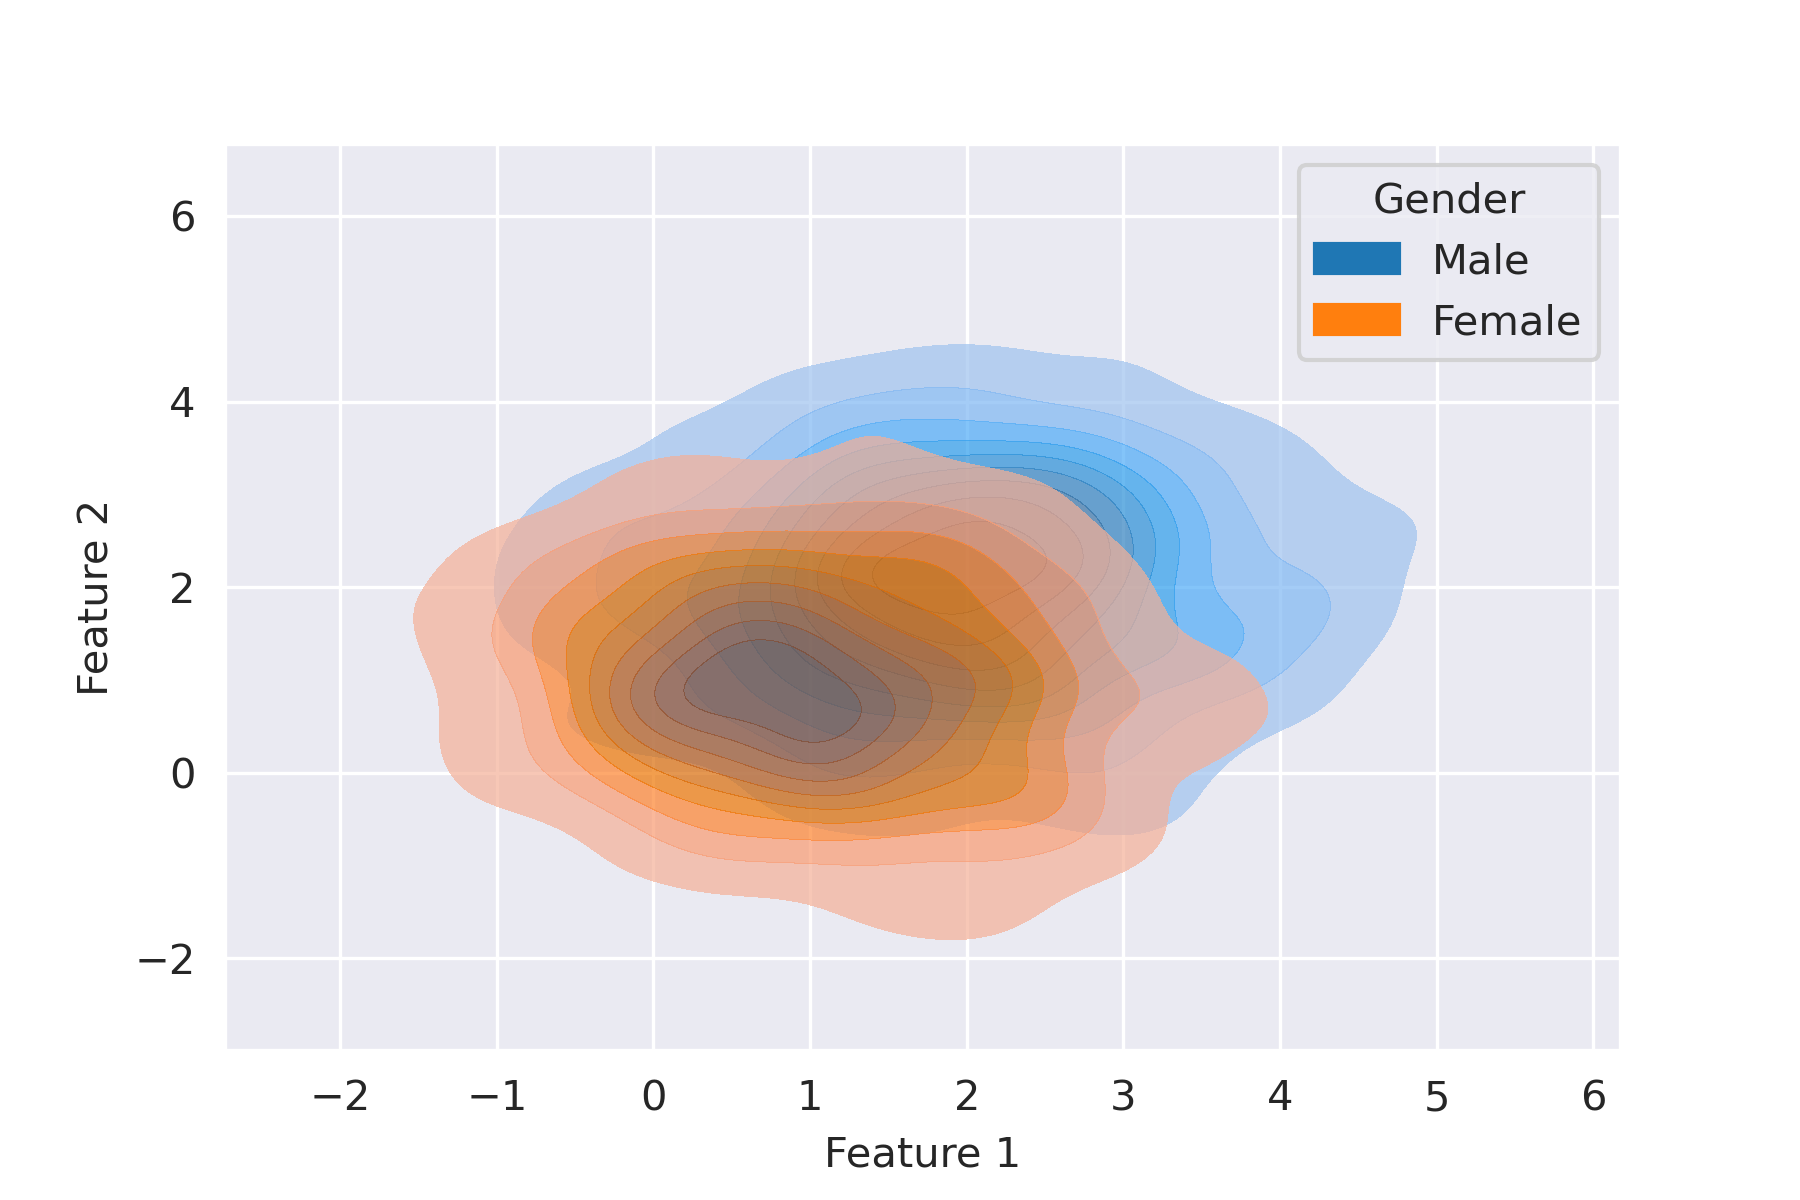
\includegraphics[width=0.49\linewidth]{figures/synthetic-gender.png}
    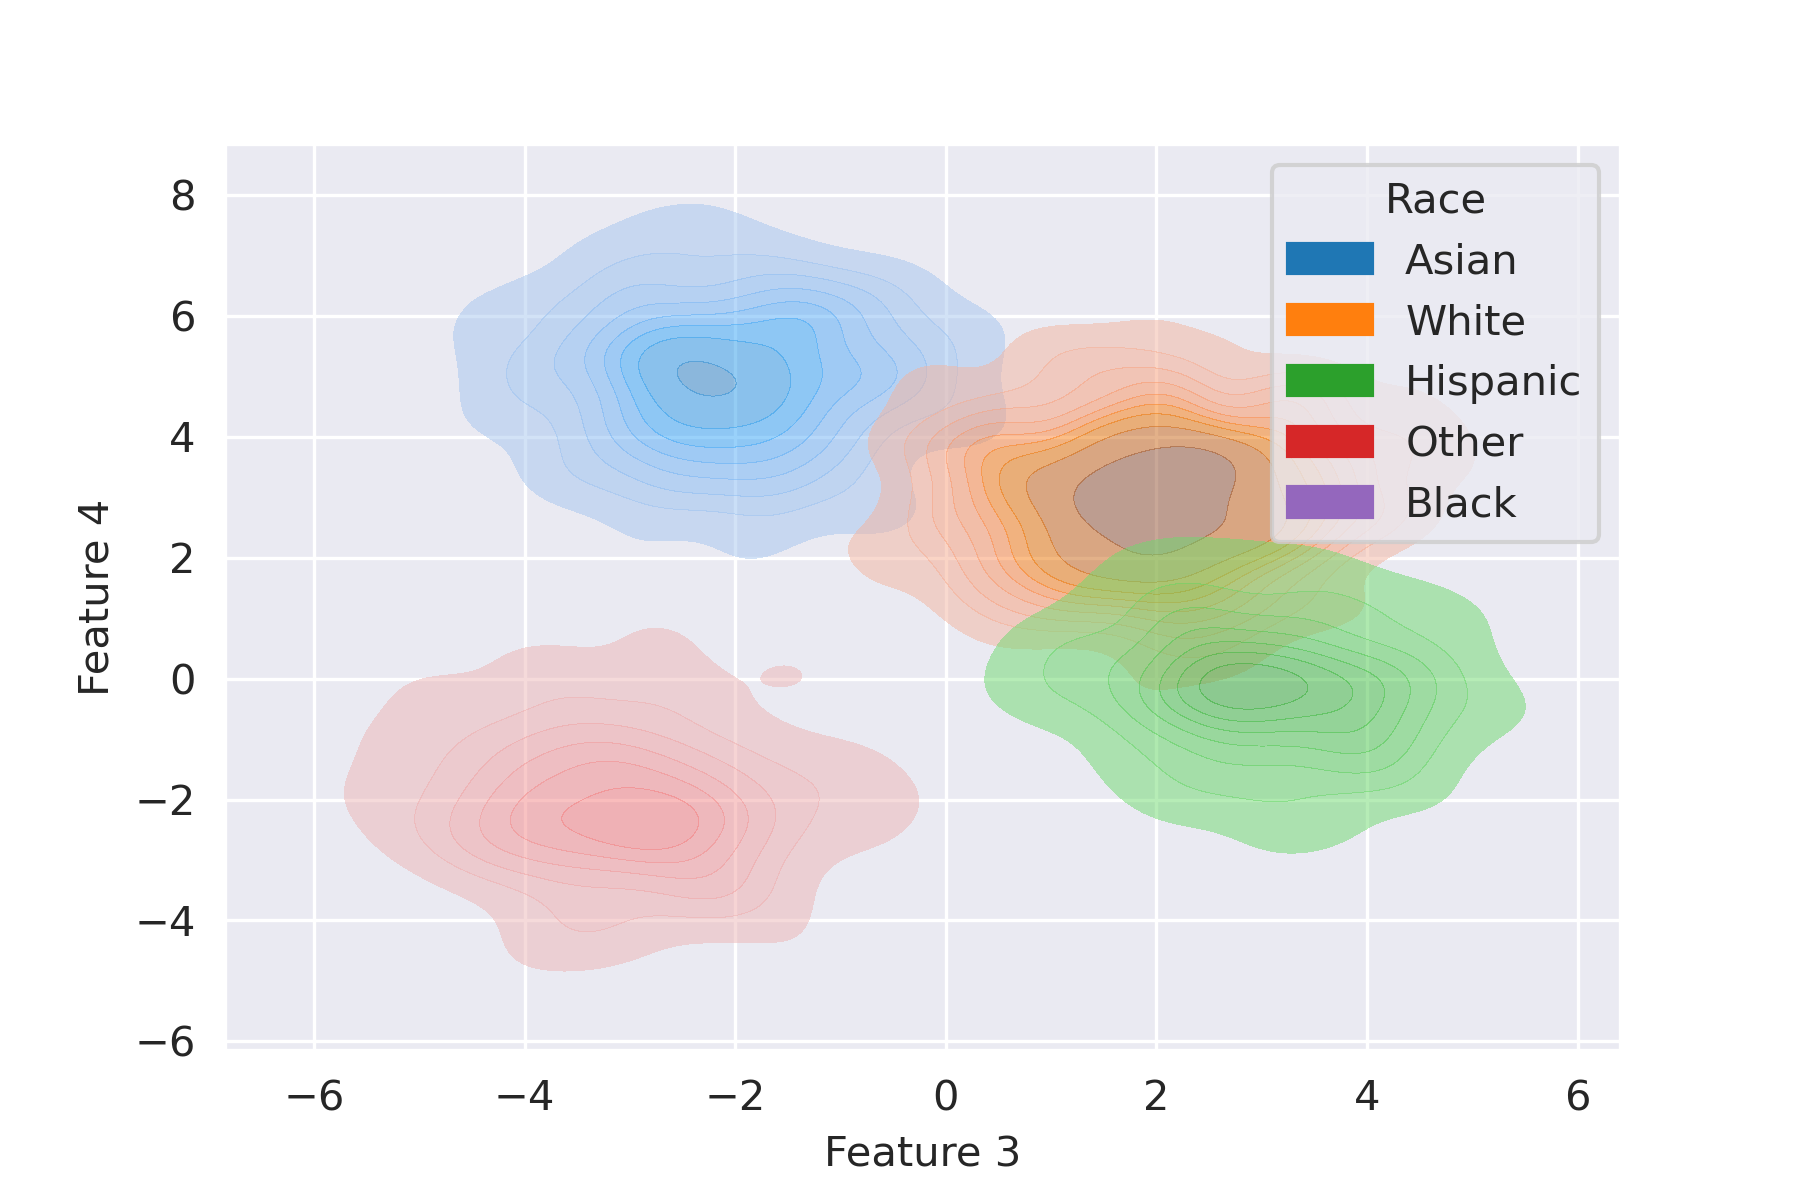
\includegraphics[width=0.49\linewidth]{figures/synthetic-race.png}
    \caption{KDE of the bivariate features of the synthetic dataset..}
    \label{fig:synthdatasetfeatures}
\end{figure}


We define a separator parameter $\Theta$ which is used to model the separation between the sensitive classes. We sample $X_1$ and $X_2$ the following way conditionally on the sensitive attribute $G_s$

\begin{equation*}
    \begin{aligned}
           X_1 | G_s = \text{Female} \sim N(1, 1) \\ 
           X_1 | G_s = \text{Male} \sim N(1 + \Theta, 1)
    \end{aligned}
\end{equation*}

And the same for $X_2$. The same principle is used for $X_3$ and $X_4$ but with a slight twist. There are $k$ races in the dataset and a random sign variable $R$ following the discrete uniform distribution over the set $\{-1, 1\}$.

\begin{equation*}
    \begin{aligned}
        X_3 | R_s = k \sim N(1 + \Theta \cdot R \cdot k, 1)
    \end{aligned}
\end{equation*}

and the same for $X_4$. Then lastly, to calculate the labels of the dataset we take the sum of all the numerical features $X = \{ X_1, X_2, X_3, X_4 \}$ and calculate the median of all the sums for each data point. If the sum is above the median, it gets labelled 1, otherwise, 0.

This can be summarised in algorithm~\ref{alg:datasetgen}

\begin{algorithm}
    \caption{Synthetic dataset generation}
    \begin{algorithmic}
        \REQUIRE $I = $ Informative. True or false, $\Theta = $ Separability, $N =$ Number of samples.
        \ENSURE $D = $ Synthetic Dataset.
        \STATE Sample $N$ samples from $G_s \sim B(1, 0.5)$
        \STATE $k = 5$
        \STATE $\boldsymbol{\tau_k} = \{ \tau_1, \dots, \tau_k \}$ with $\tau_j \sim |N(0, 1)|$
        \STATE $\theta = \boldsymbol{\tau} \cdot \frac{1}{\sum \tau_k}$
        \STATE Sample $N$ samples from $R_s \sim C(k, \theta)$
        \STATE Sample $N_{\text{Female}}$ samples from $X_1 \sim N(1, 1)$
        \STATE Sample $N_{\text{Male}}$ samples from $X_1 \sim N(1 + \Theta, 1)$
        \STATE Sample $N_{\text{Female}}$ samples from $X_2 \sim N(1, 1)$
        \STATE Sample $N_{\text{Male}}$ samples from $X_2 \sim N(1 + \Theta, 1)$
        \FORALL{$i \in \{ 1, \dots, k \}$}
        \STATE Select $R$ uniformly from the set $\{ -1, 1\}$
        \STATE Sample $N_i$ samples from $X_3 | R_s = i \sim N(1 + \Theta \cdot R \cdot i, 1)$
        \STATE Select $R$ uniformly from the set $\{ -1, 1\}$
        \STATE Sample $N_i$ samples from $X_4 | R_s = i \sim N(1 + \Theta \cdot R \cdot i, 1)$
        \ENDFOR
        \STATE $t = \sum X$ for all data points in the dataset
        \IF{$t \geq \text{Median}(X)$}
        \STATE $Y = 1$
        \ELSE
        \STATE $Y = 0$
        \ENDIF
        \STATE $D = \{G_s, R_s, X_1, X_2, X_3, X_4, Y \}$
        \RETURN $D$
    \end{algorithmic}
    \label{alg:datasetgen}
\end{algorithm}

\subsection{Fairness Performance Measure}

The performance metric used for the models up to this point is the parity score metric as described in section.~\ref{sec:demparscore}. This score is based on the notion that the likelihood of positive outcome is independent of the sensitive attributes. There is another measure that is similar to this. That is Kullback-Leibler divergence. Which according to \citet{Mackay:2003:information} is calculated as 

\begin{equation*}
    D_KL(P ||Q) = \sum_x \log\frac{P(x)}{Q(x)}
\end{equation*}

Kullback-Leibler divergence is a measure of how different two distributions $P$ and $Q$ are. It is not strictly a metric as it is not symmetric and is instead a divergence. While metrics are symmetric and linear in distance, divergences are asymmetric and generalise square distance. For our work, we want to use Kullback-Leibler divergence as a measure of unfairness. The general idea is that we want $P$ and $Q$ to denote different distributions conditional on sensitive attributes. Assume that we have a dataset with model predictions $Y$ and a binary sensitive attribute $S$. Then we define 

\begin{equation*}
    P \sim Y | S = 0
\end{equation*}

and

\begin{equation*}
    Q \sim Y | S = 1
\end{equation*}

Under demographic parity, we want $Q \perp\!\!\!\perp P , S$ and thus a Kullback-Leibler Divergence of 0. Kullback-Leibler Divergence is limited to two distributions, though there are generalisations. For this round of experiments, we limit ourselves to the binary case and calculate the divergence in the binary cases and compare them to the other metrics.

\subsection{Hypothesis Tests}

We want to perform hypothesis testing on the performance metrics of different models. Assume that we have samples of an unspecified performance metric for two different models trained on the same dataset. Let us denote the two distributions $X$ and $Y$. 

We have chosen to use non-parametric hypothesis tests, as we do not want to make assumptions on the kind of distribution the samples have. Since the samples are of model performance of two machine learning models trained on the same dataset, the samples will be dependent on each other. We therefore select the Wilcoxon signed-rank test as the testing method of choice. This test was introduced and named after \citet{Wilcoxon:1945:Biometrics}. The Wilcoxon signed-ranked test calculates the differences between the ranked samples and test whether or not the differences are symmetric around zero. We will test the following hypotheses, shown in table~\ref{tab:hypothesis}.

\begin{table}
    \centering
    \begin{tabular}{p{10cm}lll}
        \hline
        \textbf{Hypothesis} & $\boldsymbol{H_0}$ & $\boldsymbol{H_1}$ & $\boldsymbol{\alpha}$ \\
        \hline
        \hline
        FairBN ($Y$) has a better intersectional parity score than naïve Bayes ($X$) without sensitive attributes & $X = Y$ & $X < Y$ & $0.01$ \\ \hline
        FRFC ($Y$) has a better intersectional parity score than naïve Bayes ($X$) without sensitive attributes & $X = Y$ & $X < Y$ & $0.01$ \\ \hline
        FairBN ($Y$) has a better intersectional parity score than FRFC ($X$) & $X = Y$ & $X < Y$ & $0.01$ \\ \hline
        FairBN ($Y$) has a better KLD w.r.t. Gender than FRFC ($X$) & $X = Y$ & $X > Y$ & $0.05$ \\ \hline
    \end{tabular}
    \caption{List of hypothesis}
    \label{tab:hypothesis}
\end{table}

\subsection{Experiment Setup}

We ran 100 synthetic dataset generations and trained the models on the synthetic datasets and evaluated them on a test dataset. For each iteration the train-test split is $70\%$ for the training set and $30\%$ for the test dataset. We calculated the same performance metrics as in the first experiment. Additionally, we also introduce Kullback-Leibler Divergence w.r.t. Gender. 

After the performance metrics have been calculated and collected. We will visualise the distributions of the performance metrics as well as the correlation between parity score, KL Divergence and AUC score. The results are shown and discussed in section~\ref{eval:exp2}

\section{Experiment 3: Interpretable Machine Learning}

We have been able to show that the models we have trained are able to satisfy some mathematical notion of fairness in their predictions. But we want to investigate this further. By employing interpretable machine learning methods, we can try to explain how the model uses the sensitive attributes in their predictions and try to explain their behaviour. 

\subsection{Experiment Design}

For this experiment, we want to implement the following in an attempt to explain the decisions made by machine learning models

\begin{itemize}
    \item Train a baseline interpretable model and investigate the decision rules it learns.
    \item Interpret the models that are interpretable by default.
    \item Use model agnostic interpretable methods for models that are not interpretable.
\end{itemize}

In the following sections, we will describe the methods chosen to answer the above points.

\subsection{Interpreting Decision Trees}

To address the first point, we want to train a baseline interpretable model. Our choice landed on Decision Trees. According to \citet{Molnar:2020:Book} the interpretation of decision trees, while quite similar for all algorithms, differ by the kind of algorithm for building the tree is used. The interpretation described here is for the CART algorithm, which is the one implemented by Scikit-learn \cite{Pedregosa:2011:JMLR}.

The interpretation of decision trees works as follows: Starting from the root node, you go to the next nodes and the edges tell you which subsets you are looking at. Once you reach the leaf node, the node tells you the predicted outcome \cite{Molnar:2020:Book}. To calculate the feature importance. We calculate the reduction in the split. In our case, we have used entropy and information gain to evaluate splits which is defined as 

\begin{equation*}
    IG(T) = H(T) - \sum_{i = 1}^{2} \frac{n_i}{n} H(C_i)
\end{equation*}

Where $T$ is the node being split and $C_i$ is child node $i$. $H$ denotes Shannon entropy introduced by \citet{Shannon:1948:BellSystTechJ}. Go through all the splits for which the feature was used and measure how much it has reduced the information gain. Scale all the sums to $1$, then you can calculate the share of a features importance as an percentage.

We will do this for the datasets that have been used in the previous experiments to uncover what attributes are used in the model prediction.

\subsection{Interpreting naïve Bayes}

As described in section~\ref{relatedwork:naiveBayes}, the naïve Bayes classifier assumes that all features are mutually independent, conditioned on the class labels. We can therefore interpret the contributions of the different attributes through the conditional probabilities that the naïve Bayes classifier has learned \cite[p.~142]{Molnar:2020:Book}.

The way we have chosen to do this is like so: Assume that a feature $X_i$ in a dataset $\boldsymbol{X}$ is informative. Then we would expect that the likelihood on $X_i$ is very different given the class $Y$

\begin{equation*}
    P(X_i | Y = 0) \neq P(X_i | Y = 1)
\end{equation*}

In the case that $X_i$ is categorical with $k$ categories. We have a conditional dependency table on the form

\begin{equation*}
    \begin{bmatrix}
        P(X_0 | Y = 0) & P(X_0 | Y = 1) \\ 
        P(X_1 | Y = 0) & P(X_1 | Y = 1) \\
        \vdots & \vdots \\
        P(X_k | Y = 0) & P(X_k | Y = 0)
    \end{bmatrix}
\end{equation*}

Then we denote the first column $P = P(X_i | Y = 0)$ and the second column $Q = P(X_i | Y = 1)$. We assume that the more informative $X_i$ is as a feature, the difference in these distributions should increase. To calculate the feature weight we define the weight as 

\begin{equation*}
    D_{KL}(P||Q)
\end{equation*}

This should also be validated using permutation importance to compare the weights. Introduced by \ref{alg:permimp} is used and is based on the one used by Scikit-learn \cite{Pedregosa:2011:JMLR}

\begin{algorithm}
    \caption{Permutation Importance Algorithm}
    \begin{algorithmic}
        \REQUIRE $C = $ Classifier, $D = $ Test Dataset. $K = $ No of permutations.
        \ENSURE $I = $ Dataset of importances.
        \STATE Compute reference score $S$ on the test dataset $D$.
        \FORALL{columns $i\in D$}
            \FOR{$j \in \{ 1, \dots, K \}$} 
                \STATE Permute (shuffle) column $D_{i}$ and denote the corrupted dataset $\Tilde{D}_{j}$
                \STATE Compute score $s_{ij}$ on test dataset $\Tilde{D}_{j}$
                \STATE Set $I_{ij} = S - s_{ij}$
            \ENDFOR
        \ENDFOR
        \RETURN $I$ 
    \end{algorithmic}
    \label{alg:permimp}
\end{algorithm}

This algorithm returns a dataset of importances, as we want to see the distribution of importances for each feature.

\subsection{Interpreting Bayesian Networks}

Bayesian Networks are to some extent interpretable machine learning models, dependent on the complexity of the conditional dependencies. Naïve Bayes is an interpretable machine learning model and is the simplest Bayesian network. It is very intuitive for humans to explain how much each attribute contributes, as they are conditionally independent given the class label. As the complexity of the conditional dependencies increase,  they are more demanding to understand.

In our case, from the fair Bayesian network as shown in figure \ref{fig:choinetwork}. We see that the sensitive attributes are independent of the true latent dataset labels. Meaning that the sensitive attributes should not be used explicitly in the prediction. To investigate this, we want to use the permutation importance algorithm to see how important the features are for getting accurate predictions. We will also apply counterfactual generation described in section~\ref{sec:counterfactuals} on the fair Bayesian network for further interpretability.

\subsection{Interpreting Fair Random Forest}

Random Forests are not interpretable as the many different trees used for predictions are not immediately intuitive to explain, and in many cases so many that the interpretation is incomprehensible in human terms. Therefore, one has to resort to model agnostic interpretability methods if one wants to gain some insight. We have chosen to use feature importance here as well in an effort to understand the model.

There is one challenge with the approach by \citet{Antonio:2021:arXiv}, and that is the fact that the sensitive attributes are only used during training of the model. Meaning that one cannot infer how the model uses the sensitive attributes neither using the permutation importance method nor counterfactual generation. We will resort to investigating how the model uses the non-sensitive attributes in their prediction to investigate how the model achieves fairness.

\subsection{Counterfactuals}
\label{sec:counterfactuals}

According to \citet{Molnar:2020:Book}, a counterfactual explanation should describe the smallest change to the feature values that changes the prediction to a predefined output. In our case for the Adult and the COMPAS dataset, we want to generate the smallest changes to get a positive outcome (being classified as high income or not likely to reoffend). Counterfactuals should follow these criteria

\begin{itemize}
    \item Counterfactuals should be as similar as possible to the instance regarding feature values.
    \item Counterfactual instances should have feature values that are likely.
    \item Change as few features as possible.
\end{itemize}

Various methods exist for generating counterfactuals, while we will get inspiration from the method proposed by \citet{Dandl:2020:PPSN}, specifically the NSGA-II algorithm introduced by \citet{Pratap:2002:IEEE.Trans.Evol.Comput.}. We want to generate counterfactuals that satisfy the following objectives 

\begin{equation*}
    o_1(\hat{f}(\boldsymbol{x}), Y') = 
    \begin{cases}
        0 & \text{if} \hat{f}(\boldsymbol{x}) \in Y' \\
        \underset{y' \in Y'}{\text{inf}} |\hat{f}(\boldsymbol{x}) - y'0|, & \text{else} \\
    \end{cases}
\end{equation*}

Which is the distance between the desired prediction $y'$ and the predicted value $\hat{f}(\boldsymbol{x})$.  The second objetive $o_2$ reflect that counterfactuals should be as equal to the instance $\boldsymbol{x}$ that we want to flip the prediction for

\begin{equation*}
    o_2(\boldsymbol{x}, \boldsymbol{x'}) = \frac{1}{p} \sum_{j=1}^{p} \mathbb{I}_{x_j \neq x'_j}
 \end{equation*}

Which uses the indicator function,  as the models implemented in pgmpy uses categorical data. Numerical values are also categorical as they are discretised. Next, we introduce $o_3$ which measures the amount of features that have been changes.

\begin{equation*}
    o_3(\boldsymbol{x}, \boldsymbol{x'}) = ||\boldsymbol{x} - \boldsymbol{x'}||_0 = \sum_{j=1}^{p} \mathbb{I}_{x_j \neq x'_j}
\end{equation*}

Lastly, we want the counterfactual to have attributes that are likely to occur. We measure this by searching for the closest sample in the training dataset and calculate the distance between the candidate and the closest point.

\begin{equation*}
    o_4(x', X^\text{obs}) = \frac{1}{p} \sum_{j=1}^{p} \mathbb{I}_{x_j \neq x^{[1]}_j}
\end{equation*}

And we try to minimise all these objective functions at once. To do this we will have to resort to a genetic algorithm as we do not want to collapse the four objectives into one but optimise all at the same time.

\subsection{Nondominated Sorting Genetic Algorithm: NSGA-II}

The NSGA-II algorithm introduce by \citet{Pratap:2002:IEEE.Trans.Evol.Comput.} works as a four step iterative algorithm. The steps are as follows:

Initially, we generate a parent population that consists of $N$ number of mutated copies of $\boldsymbol{x}$, the data point we want to change the outcome for. The mutations in the beginning are quite extensive so that we explore the optimisation space thoroughly. Then, we use fast-non-dominated-sort algorithm \cite[p.~184]{Pratap:2002:IEEE.Trans.Evol.Comput.} to rank the population into frontiers. 

Then, we add each frontier in decreasing order into the new population $P_\text{new}$ until there is no room to add the next frontier. Then we apply the crowding-distance-assignment method to add the remaining number of slots from the last frontier into $P_\text{new}$ \cite[p.~185]{Pratap:2002:IEEE.Trans.Evol.Comput.}

We then have a new population $P = P_{\text{new}}$ and we create a new generation $R$ which consists of mutated samples from $P$. We then rank $R \cup P$ using nondominated sorting and reiterate the steps above until the specified amount of iterations is completed.

The code for NSGA-II is added to the classes \emph{interpretableNaiveBayes} and \emph{latentLabelClassifier} as a method in Forseti.